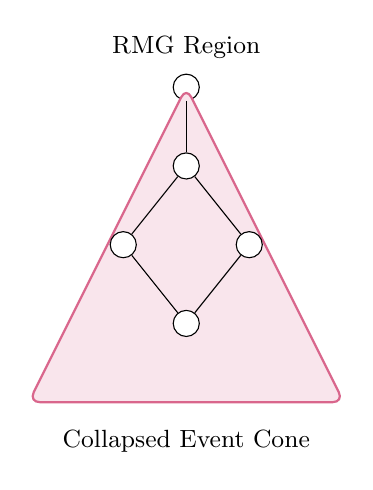
\begin{tikzpicture}[
    cone/.style={draw=purple!60, thick, fill=purple!10, rounded corners},
    smallnode/.style={circle, draw=black, fill=white, minimum size=5pt},
    arrow/.style={->, thick}
]

% Macro node
\node[smallnode] (macro) at (0,0) {};

% Cone
\draw[cone] (-2,-4) -- (0,0) -- (2,-4) -- cycle;

% Micro nodes inside
\node[smallnode] (m1) at (0,-1) {};
\node[smallnode] (m2) at (-0.8,-2) {};
\node[smallnode] (m3) at (0.8,-2) {};
\node[smallnode] (m4) at (0,-3) {};

\draw (macro) -- (m1);
\draw (m1) -- (m2);
\draw (m1) -- (m3);
\draw (m2) -- (m4);
\draw (m3) -- (m4);

% Label
\node at (0,0.5) {\small RMG Region};
\node at (0,-4.5) {\small Collapsed Event Cone};

\end{tikzpicture}